\pdfbookmark{Общая характеристика работы}{characteristic}             % Закладка pdf
\section*{\centering DISSERTATION TOPIC}

\renewcommand{\figurename}{Figure}
\renewcommand{\tablename}{Table}
\renewcommand{\bibtitlefull}{References}

Modern deep reinforcement learning methods (RL) can solve optimal control and planning tasks without a priori information about the problem. Learning is performed through trial and error as the agent interacts with the environment and learns to optimize its actions to maximize the expected reward. This formulation closely resembles how humans learn, and can be considered as one of the approaches to creating artificial general intelligence \cite{reward_is_enough}. Deep reinforcement learning was applied for the first time to control a virtual agent in an Atari 2600 game-based environment in 2013\cite{mnih2013atari}. It has been shown that RL can control the agent based on visual information at the human level. Since then, the topic of machine learning with reinforcement has received more and more attention. Reinforcement learning is effective in many complicated tasks such as playing chess~\cite{alphazero}, go~\cite{alphago}, and StarCraft II~\cite{alphastar}. These impressive results have become possible due to the development of both RL methods and computer technology, since successful training of deep RL agents requires a huge number of interactions with the environment. The research carried out in this work is mainly focused on the development of reinforcement learning methods applicable to the control of real robotic devices. The creation of algorithms capable of making decisions in the real world, self-learning, and not requiring large amounts of human-labeled data, can lead to explosive growth in collaborative robotics, self-driving cars, and the field of virtual assistants.

At present, the scope of application of RL methods is limited. The main limiting factor is the large amount of data needed to train the agent. To leverage this problem, the agent is often trained in a virtual environment --- a simulator, and then transferred to a physical installation. This setting leads to a second problem --- a difference between observations and the dynamics of the environment in the simulation and the reality, which results in a significant decrease in the performance of the agent in the real world. Another problem arises when an agent is trained directly on a physical robot --- the ability of the agent to perform actions that could break the robot should be limited during the learning process without a large restriction on the agent's ability to explore the environment. Moreover, many practical tasks can be viewed as a hierarchy of subtasks. While one part of the subtasks can be effectively solved by classical methods, the other part requires more complex learning methods. This leads to the need to combine neural networks and classical approaches within a single hierarchical agent.

\underline{\textbf{Actuality.}}  One of the most promising applications for reinforcement learning methods is robotics. Modern robots are already replacing humans in strictly controlled environments such as manufacturing lines because it is possible to develop a program that takes into account all possible environment states. In contrast, in the everyday life, it is important to act in conditions of uncertainty. In such cases, the optimal behavior is difficult to program, but it can be learned through interaction with the environment. However, in order to apply reinforcement learning methods to control physical robots, one needs to solve a number of challenges such as reducing the number of examples needed for training; increasing the efficiency of transferring models trained in simulation to the real world; developing algorithms capable of solving problems in the absence or sparse reward function. 

In the present dissertation, we developed methods with would mitigate limitations of reinforcement learning algorithms in a real world tasks. We evaluate the performance of our algorithms on a set of important practical applications and propose a novel application for reinforcement learning methods --- alignment of an optical interferometer. 
For the first time, we developed a reinforcement learning method for the alignment of an optical Mach-Zehnder interferometer \cite{interferobot, v2}. To align an interferometer, the agent must be capable of sampling actions with different amplitudes --- large actions at the beginning and small, precise actions at the end of the alignment process. The size of the actions at the beginning of an episode can be more than 100 times bigger than at the end. This problem is not frequent in usual RL benchmarks but is important for practical applications. Also, the agent trained in the simulation must be robust to optical noises in the input images when deployed at the experimental setup. Interferometers are a common part of most setups in experimental optics. Alignment of the experimental setup is one of the most labor-intensive phases in experimental optics. Fine-tuning hundreds of optical elements such as lenses, mirrors, and attenuators require a lot of experimental experience and takes many hours even for an experienced specialist. Automation of the alignment process will greatly increase the performance of optical experiments. The developed method uses images from cameras and adapts to the parameters of a particular setup. The proposed method is significantly superior to a human in terms of quality and speed of interferometer alignment.

A similar task of continuous control arises in quadruped robots. We considered the task of controlling the movement of a quadruped Unitree A1 robot\cite{rl_unitree}. For successful learning of RL algorithms, it is important to specify the reward function. With a carelessly given reward function, an agent can learn a suboptimal strategy. We propose a reward function with penalties for the non-optimality of the agent's strategy increasing according to the schedule. The proposed reward function was applied to train the RL agent to control the movement of the Unitree A1~\cite{unitree} robot with given parameters such as angular and linear velocities. The proposed reward function encourages the agent to learn safe and smooth movement at a given speed. In this case of a robot with many degrees of freedom, the use of reinforcement learning has significant advantages over classical algorithms, since the agent can independently learn the optimal strategy based only on the scalar reward function. The optimal strategy should filter out the noise in the observations well, not require an excessive amount of data for training, and not perform actions that could damage the robot. The results of testing the trained agent showed that it is able to perform well in the simulation.

The next challenge in the application of reinforcement learning methods in the real life is to combine them with algorithmic approaches to solve complex problems. As part of this work, we propose a hierarchical algorithm that combines reinforcement learning, classical algorithms on graphs, and expert knowledge. The strategy is built from basic skills designed to solve specific problems, and the choice of skill is based on the current state. The developed algorithm was applied to control a virtual agent in the NetHack \cite{nethack} environment. This environment is one of the most difficult test environments for reinforcement learning algorithms. The average episode length in NetHack is 100,000 steps, which is 50 times longer than in StarCraft II. NetHack is also a procedurally generated environment, which means that an agent can rarely be in the same state more than once. The large space of actions and different states of the environment means that most of the methods used in reinforcement learning to explore the environment do not work in this setting. The developed method made it possible to effectively apply reinforcement learning to this problem and won first place in the competition held by Google DeepMind and Facebook AI Research as part of the NeurIPS Competition track 2021 conference. This approach can be used to design systems that combine machine learning and classical algorithms.

\underline{\textbf{The aim}} of this work is the development of machine learning methods for the control of robots in real-world tasks.

We formulate the following \underline{\textbf{goals of this research}}:
\begin{enumerate}[beginpenalty=10000] % https://tex.stackexchange.com/a/476052/104425
  \item Development of a simulator of Mach-Zehnder interferometer
  \item Formulation of an optical interferometer alignment in terms of Markov decision process; selection of the a reward function; definition of action and observation spaces; selection of hyperparameters
  \item Development of reinforcement learning algorithm capable of operate with actions of different magnitude and robust to optical noises
  \item Development of software complex to align a physical a setup of optical interferometer
  \item Development of a curriculum based method with penalties increasing according to a schedule and training an RL algorithm to control the speed of a quadruped robot
  \item Development of a hierarchical method that combines algorithmic and neural approaches and its application to the NetHack environment
\end{enumerate}


\underline{\textbf{Scientific novelty:}}
\begin{enumerate}[beginpenalty=10000] % https://tex.stackexchange.com/a/476052/104425
  \item We proposed a reinforcement learning method which can operate actions of different magnitude and robust to optical noises. This method was for the first time applied to align the optical interferometer
  \item For the first time, we created a hardware-software complex for tuning an optical interferometer based on images from a camera based on machine learning with reinforcement
  \item We developed an original method for learning a strategy to control the movement of a quadruped robot with desired speed
  \item We performed an original study on the applicability of a hierarchical algorithm combining neural and algorithmic policies for the Nethack game.
\end{enumerate}

\underline{\textbf{Theoretical and practical significance}} of the work is:
\begin{enumerate}[beginpenalty=10000] % https://tex.stackexchange.com/a/476052/104425
  \item The automated approach to the alignment of the optical interferometer proposed in the dissertation will significantly speed up the conduct of physical experiments and reduce the need for manual labor
  \item The developed algorithms for controlling virtual agents can then be applied in robotics, self-driving cars and virtual assistants
\end{enumerate}

\underline{\textbf{Research methods.}} In the work we applied methods of machine learning, computer vision, deep reinforcement learning, software development, linear algebra, general physics and optics.

\section*{\centering{KEY RESULTS}}

\underline{\textbf{The main defense points:}}
\begin{enumerate}[beginpenalty=10000] % https://tex.stackexchange.com/a/476052/104425
  \item A reinforcement learning method capable of handling actions of various scales and resistant to optical noise. The developed method makes it possible to adjust the optical interferometer without human intervention, based solely on images of the interference pattern. The proposed method does not use a priori information and is able to independently learn for a specific installation.
  \item Hardware-software complex for automatic tuning of an optical interferometer. The speed and accuracy of tuning using the developed method significantly exceeds manual tuning.
  \item A reinforcement learning method for policy learning for controlling the movement of a quadruped robot with a given linear and angular velocity.
  \item Hierarchical algorithm combining algorithmic and neural approaches. The algorithm was tested in the NetHack environment.
\end{enumerate}

\underline{\textbf{Author’s contribution to the study.}} The author personally developed a simulator of the optical interferometer; software and hardware complex for launching and testing a trained agent on the experimental setup; a method for tuning an interferometer with a reinforcement machine learning algorithm using a discrete action space. The author has been actively involved in the development of a machine learning method for alignment of the interferometer using a continuous action space. The author personally proposed and implemented a reward function that allows learning a strategy to control the movement of a walking robot at a given speed. The author personally proposed and implemented the idea of an algorithm for playing Nethack in the form of a hierarchical agent that combines machine learning with reinforcement and an algorithmic approach. 

\section*{\centering{PUBLICATIONS AND APPROBATION OF RESEARCH}}

\paragraph{First-tier publications} 
\begin{refsection} 
    \nocite{confbib1}
    \printbibliography[heading=none]
\end{refsection}

\paragraph{Second-tier publications}
\begin{refsection} 
    \nocite{confbib4}
    \printbibliography[heading=none]
\end{refsection}

\paragraph{Other publications}
\begin{refsection} 
    \nocite{confbib2}
    \nocite{confbib3}
    \nocite{progbib1}
    \printbibliography[heading=none]
\end{refsection}

\expandafter\def\csname blx@maxbibnames\endcsname{3}% sorokin reset et.al max names

\paragraph{Reports at conferences and seminars}
\begin{enumerate}[labelindent=3pt, labelsep=10pt, topsep=10pt, itemsep=5pt]
    \item 34-th annual international conference Neural Information Processing Systems (NeurIPS 2020) (\textbf{spotlight talk})
    \item 29-th annual international conference on laser physics LPHYS 2021
    \item 5-th international Conference on Robot Learning (CoRL) 2021
    \item 35-th international conference Neural Information Processing Systems (NeurIPS 2021, Competition track)
    \item International conference on quantum technology ICQT 2021
    \item International conference on artificial neural networks Neuroinformatics 2022
\end{enumerate}

\paragraph{Participation in scientific projects}
\begin{enumerate}[labelindent=3pt, labelsep=10pt, topsep=10pt, itemsep=5pt]
    \item Grant UMNIK <<Development of an automatic alignment system for an optical interferometer based on machine learning>> № 120ГУЦЭС8-D3/56352 от 21.12.2019

\end{enumerate}


\underline{\textbf{The reliability}} of the results obtained is ensured by complex testing of the proposed method of automated tuning optical interferometer, carried out at RQC. According to the results competition held by Google DeepMind and Facebook AI Research, the developed method of managing an agent in the NetHack environment has surpassed the rest approaches using neural networks.

%\underline{\textbf{Объем и структура работы.}} Диссертация состоит из~введения,
%четырех глав, заключения и~приложения. Полный объем диссертации
%\textbf{ХХХ}~страниц текста с~\textbf{ХХ}~рисунками и~5~таблицами. Список
%литературы содержит \textbf{ХХX}~наименование.

\pdfbookmark{Содержание работы}{description}                          % Закладка pdf
\section*{\centering CONTENTS}
The \underline{\textbf{introduction}} substantiates the actuality of the research conducted in the present dissertation. We present an overview of the literature which shows the great potential of deep reinforcement learning methods in decision-making tasks. We formulate goals and tasks for the present work. We present the scientific novelty and practical significance of the results of the work. The following chapters first describe the general principles of reinforcement learning methods. Then we present modern reinforcement learning methods which achieve state-of-the-art results in various benchmarks. In the first chapter, we describe the task of alignment of an optical interferometer in terms of reinforcement learning. After, we present our methods to learn reinforcement learning agents to align the interferometer using discrete and continuous action spaces and the results of the evaluation of trained models on a physical interferometer setup. The second chapter introduces the task of control of a quadruped robot. We present the proposed method for learning a policy for locomotion with target speed. The third chapter formulates the need for complex test problems to develop and test the generalization ability of reinforcement learning methods. We formulate challenges, which makes the game of Nethack one of the most difficult test environments for reinforcement learning methods. Then we present the developed algorithm and evaluate its performance. In conclusion, the main results obtained during the preparation of the dissertation research are summarized, indicating their novelty and practical significance.


The \underline{\textbf{first chapter}} is devoted to an overview of reinforcement learning methods (RL) and their applications in robotics. It formulates the RL problem --- maximization of the expected total discounted reward obtained in interaction with the environment. Schematically, this interaction is shown in fig. \ref{fig:rl_setting}. In the fig.\ref{fig:rl_setting} an agent interacts with the environment through actions and receives from the environment tuple of next state, reward, and termination flag. 

\begin{figure}[ht]
    \centerfloat{
        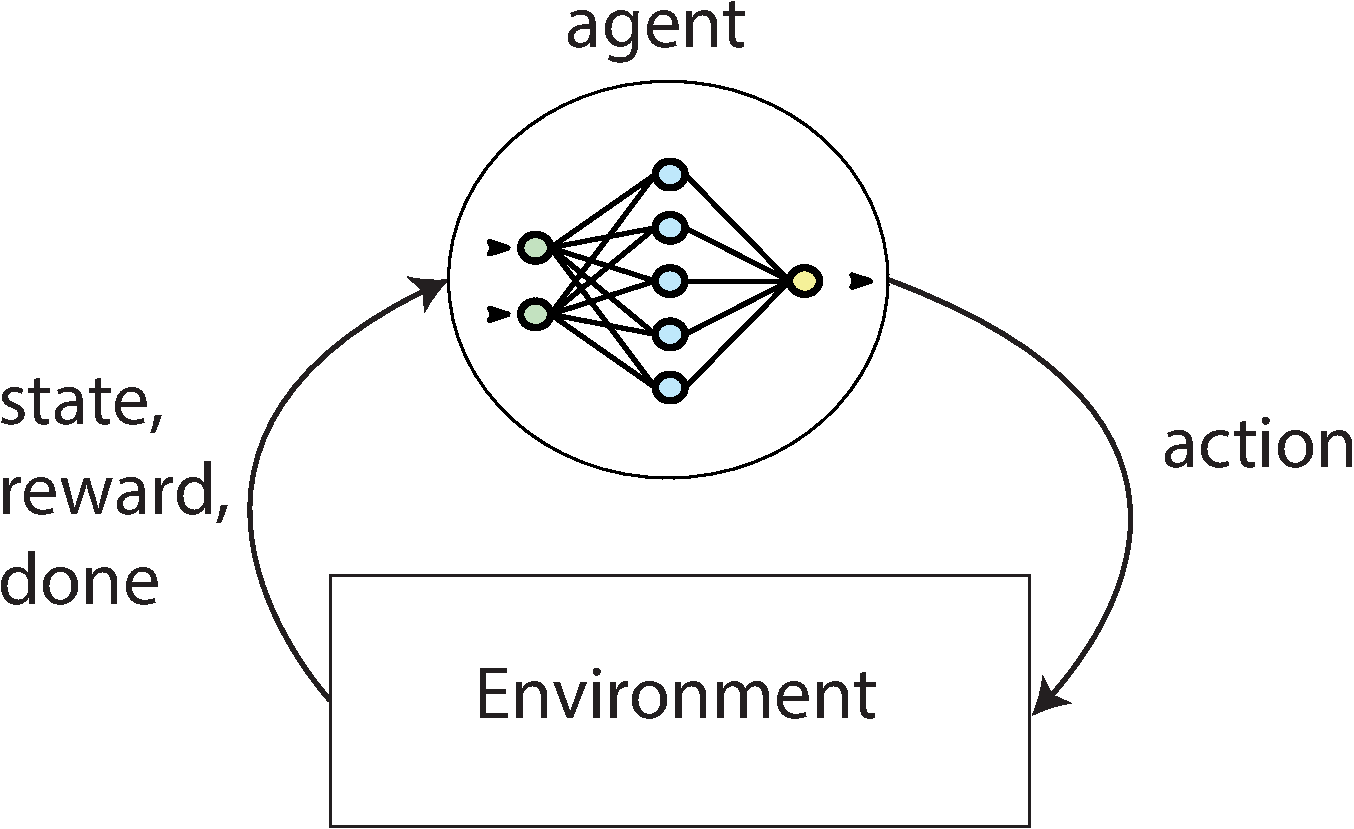
\includegraphics[width=0.6\linewidth]{images/rl_setting}
    }
    \caption{Interaction of RL agent and environment.}\label{fig:rl_setting}
\end{figure}

Expectation of the total discounted reward is calculated along trajectories sampled from the current policy of the agent:

\[
E_{\tau \sim \pi(\theta)} [G(\tau)] = E_{\tau \sim \pi(\theta)} [R_0 + \gamma R_{1} + \gamma ^ 2 R_{2} + ...] = E_{\tau \sim \pi(\theta)} [\sum_{t=0}^{T - 1} \gamma ^t R_{t}]
\]

The interaction between the agent and the environment is considered under the assumption of a Markov decision process. The Markov property says that the next state of the environment and the reward received by the agent depend only on the previous state of the environment and the action taken by the agent in this state. Given this assumption, the optimal strategy of an agent depends only on the current state of the environment, which allows using the Bellman optimality equation. The Bellman optimality equation expresses the relationship between the optimal strategy in two successive states of the environment $s$ and $s'$

\[
	V^*(s) = \max_{a \in \mathcal{A}} E(r_{t + 1}(s, a, s') + \gamma V^*(s_{t + 1}))
\]
where $V^*(s)$ (V-function) - expectation of total discounted reward in state $s$ under the condition of optimal strategy, $\gamma$ is the discounting factor. Equivalently, the Bellman equation can be expressed as follows: 

\[
	Q^*(s, a) = E(r_{t + 1}(s, s', a) + \max_{a \in \mathcal{A}} \gamma Q^*(s_{t + 1}, a))
\]
where $Q^*(s, a)$ (Q-function) - expectation of total discounted reward in state $s$ under the condition of action $a$ and following the optimal strategy in the next state $s'$.

Next, we will consider the main reinforcement learning algorithms. Conventionally, they can be divided into two large classes of off-policy methods and on-policy methods. Off-policy methods are based on maximization of the Q-function using the time difference method. Such methods can use data obtained by an arbitrarily policy. Due to this, off-policy methods usually require less data, but may be unstable during training. On the other hand, on-policy methods which can use only data obtained by the current policy are more stable, but require significantly more training data. 

Then we consider tasks with \textbf{sparse reward}. In such environments, the probability that an agent following random policy will find a non-zero reward and thus receive a positive learning signal is negligible. In this case, approaches called intrinsic motivation are used. The general idea of these methods is to reward the agent for discovering new states, which would motivate it to efficiently explore the environment.

The \textbf{meta-learning} algorithms are discussed next. Generally, reinforcement learning methods are designed to solve a concrete task and cannot be easily generalized to similar problems. In order to train an agent to solve a similar task, its training should be started from the beginning. Meta-learning algorithms allows to train an agent that can adapt to a distribution of tasks. 

Next we discuss \textbf{hierarchical reinforcement learning}. The main idea of hierarchical reinforcement learning is to construct a policy as a hierarchy of skills, in which the lower-level policies solve sub-tasks that are used by the upper-level policy to solve more complex problems. Such a decomposition can be useful in wide range of problems. For example, in the task of controlling a walking robot, the lower level policy can be trained to walk in a target direction, while the upper level policy uses this skill to move the robot to a given point.

At the end of the chapter, we discuss the application of reinforcement learning methods in the problems of controlling robots. Recently, RL methods have achieved outstanding results, such as solving a Rubik's Cube with a robotic arm \cite{rubic} and even controlling a fusion reactor \cite{tokomak}. Compared to methods based on classical control algorithms such as inverse kinematics, machine learning algorithms are able to adapt to the parameters of the robot and, consequently, work in conditions where these parameters are not precisely known.

\underline{\textbf{Second chapter}} is devoted to the development of a software and hardware complex for aligning an optical interferometer based reinforcement learning. At the beginning of the chapter, we discuss the physical principles of an optical interferometer. The optical interferometer is based on the principle of light interference - when two coherent light waves are superimposed, light oscillations of different amplitudes occur at different points in space. Depending on whether the waves are superimposed in-phase or in anti-phase, the interference leads to an increase or decrease in the total amplitude of the oscillations. Within the framework of this work, the interference of two light beams emitted by one laser light source was considered. In this case, the interference pattern looks like a series of bright and dark fringes visible to the naked eye. Schematically, the interference pattern obtained by superimposing two light beams with directions given by the wave vectors $k1$ and $k2$ is shown in the fig. \ref{fig:two_beam_interf}.

\begin{figure}[ht]
    \centerfloat{
        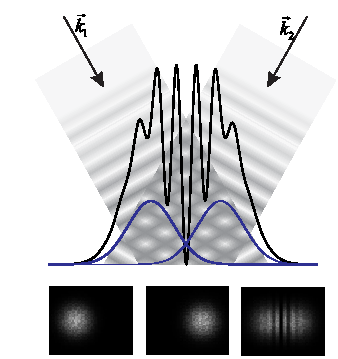
\includegraphics[width=0.5\linewidth]{images/two_beam_inreference.pdf}
    }
    \caption{
    One-dimensional slice of the interference pattern obtained with incomplete overlap of two coherent laser beams with wave vectors denoted by ~k1 and ~k2. The wavefront is shown using a gray gradient; blue lines show the intensities of each beam (not to scale); the black line shows the intensity of the interference pattern. The 2D interference patterns corresponding to the 1D case are shown below.}
\label{fig:two_beam_interf}
\end{figure}

The interferometer uses the principle of interference to accurately measure the relative phase difference between two coherent laser beams. The interferometer is one of the essential instruments used in optical experiments. For instance, the Fabry-Pierrot interferometer is used in spectroscopy \cite{fabry-perot1899}; modern gravitational wave detectors LIGO and VIRGO \cite{LIGO, VIRGO} use a Michelson interferometer; Sagnac interferometer is used in navigation systems \cite{Kandpal2000}; The Mach-Zehnder interferometer is the main tool for conducting modern experiments in quantum optics \cite{Ourjoumtsev2006, Sychev2017}.

\begin{figure}[ht]
    \centering
     \begin{subfigure}[b]{0.45\linewidth}
         \centering
         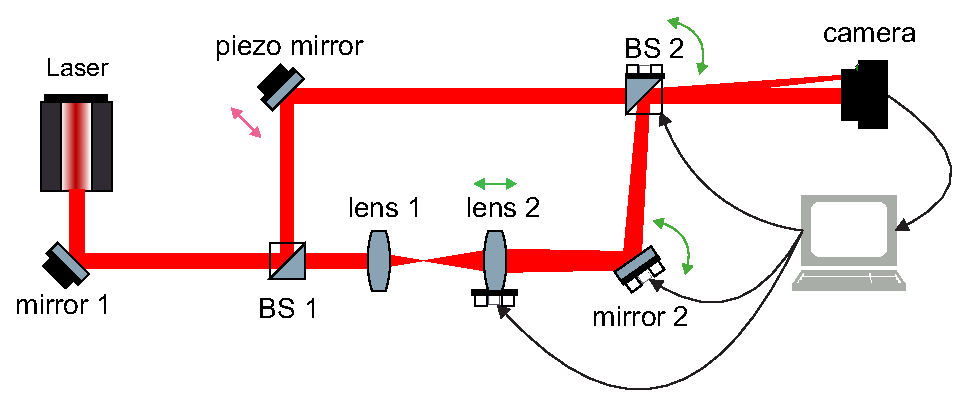
\includegraphics[width=1\linewidth]{interferobot_scheme}
     \end{subfigure}
     \centering
     \begin{subfigure}[b]{0.45\linewidth}
         \centering
         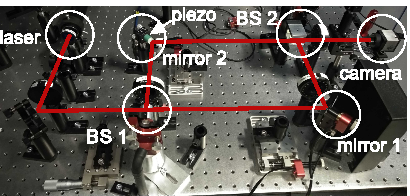
\includegraphics[width=1\linewidth]{interf_real_1}
     \end{subfigure}
    \caption{
     Principal scheme and experimental setup of Mach-Zehnder interferometer.}
\label{fig:interf_scheme_1}
\end{figure}

Next we consider Mach-Zenhder interferometer shown in fig. \ref{fig:interf_scheme_1}. In the scheme shown in the fig. \ref{fig:interf_scheme_1} the laser beam is divided into two by the first beam splitter (BS 1). Then the two beams propagate along the two arms of the interferometer and are combined at the second beam splitter (BS 2). The resulting interference pattern is observed by a digital camera. To control the mirror (mirror 1), beam splitter (BS 2) and lens (lens 2) we use optomechanical shifts. The mirror and the beam splitter shifts can rotate in two planes, while the lens shift moves linearly. The control is performed by a PC using an actuator. The goal of interferometer alignment is to precisely match the two beams after passing through the interferometer arms so that their center positions, k-vector directions, and wavefront curvatures match. The interferometer is aligned based on the interference pattern observed on the camera. An important part of the observations is the temporal dynamics of the interference fringes observed due to the piezo mirror (mirror 2) which moves periodically with an amplitude of the order of a wavelength. In our experiment, the time of the forward pass of the piezo mirror is longer than the time of the backward pass, which makes it possible to guess not only the absolute of the angle between the k-vectors, but also its sign.

Despite the apparent simplicity, the process of alignment of the interferometer is laborious. Firstly, this is due to the fact that each movement of the mirror (mirror 1) and beam splitter (BS 2) leads to a simultaneous change in both the position on the camera and the direction of the lower beam. Thus, when the beams are moved together, their parallelism is violated and vice versa. Secondly, the interference pattern observed by the camera may contain optical noise, aberrations and dust particles as shown in \ref{fig:noise}(a). In the third, optomechanical shifts that control the positions of optical elements have a significant hysteresis and limited sensitivity.

\begin{figure}
\centering
  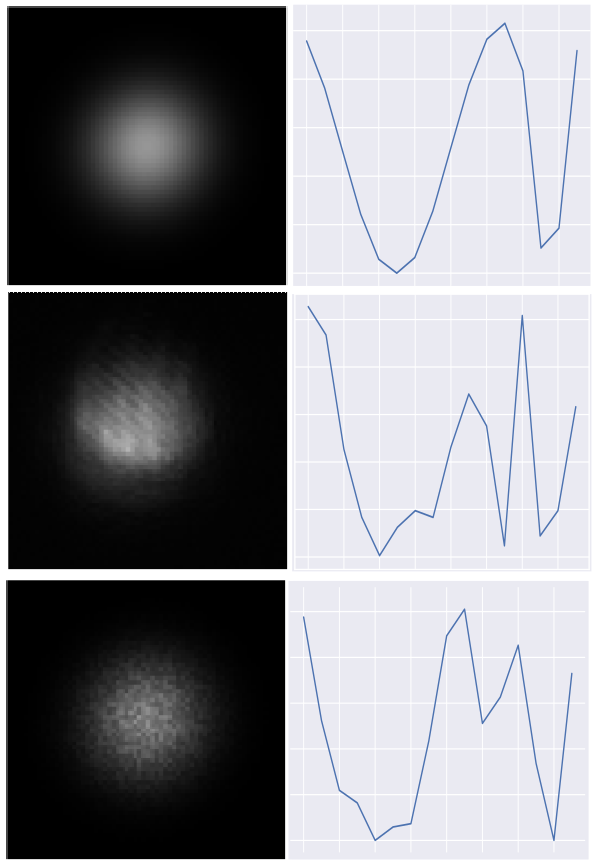
\includegraphics[width=0.5\linewidth]{beamsamples}

\caption{Laser beams: (a) experimental; (b) simulation with Gaussian amplitude profile; (c) simulation with noise. In fig. (a), fringes are visible due to the resonator effect.}
\label{fig:noise}
\end{figure}

After, we present a computer model of Mach-Zehnder interferometer constructed on the basis of interference principles, which can simulate images obtained on the camera of an optical interferometer with an arbitrary arrangement of optical elements - mirrors and lenses. In our model, laser beams in cross section are described by the Gaussian function. The vector of the electric field strength at the point $(x,y,z)$ for the beam propagating along the upper arm of the interferometer is given by the expression:

\begin{equation}
    E_u={\textrm Re}\left[\exp \left(-\frac{x^{2}+y^{2}}{r_u^{2}(z)}\right) \exp \left(-i\left(k_{z} z+ k\frac{x^2+y^2}{2\rho^2_u(z)} + \phi_{\textrm piezo}(t)\right)\right)\right]
    \label{eq:upper_beam}
\end{equation}

The vector of the electric field strength for the beam propagating along the lower arm of the interferometer is given by:

\begin{multline}
    E_l={\textrm Re}\biggl[\exp \left(-\frac{\left(x-x_{0}\right)^{2}+\left(y-y_{0}\right)^{2}}{r_l^{2}(z)}\right)  \cdot \\
    \exp \left(-i\left(k_{x} x+k_{y} y+k_{z} z + k\frac{x^2+y^2}{2\rho^2_l(z)} z\right)\right)\biggr]
    \label{eq:lower_beam}
\end{multline}

where $(x_0, y_0)$ is the position of the center of the lower beam [the center of the upper beam is assumed to be $(x,y)=(0,0)$], the beam propagates along the $z$ axis, $r(z)$ beam radius, $\rho(z)$ wavefront curvature radius, $(k_x,k_y,k_z)$ wave vector with $k=\sqrt{k_x^2+k_y^2+k_z^2 }=2\pi/\lambda$, and $\phi_{\textrm piezo}(t)$ is the phase shift due to the periodic movement of the piezo mirror. We use the paraxial approximation $k_z \gg k_x, k_y$.

Prior the beam splitter (BS 1), the two beams have identical parameters. To calculate the beam parameters after passing through the lens system we use the formalism of ABCD matrices. In the ABCD method the beam is characterized by the complex-valued parameter $\dfrac{1}{q} = \dfrac{1}{\rho} - \dfrac{i \lambda}{\pi r^2}$ and the change in the beam parameters when passing through the system lenses is written as follows $q'=\dfrac{A q+B}{C q+D}$,
where the resulting system matrix $M_{total}$ is calculated as the product of the matrices $M_{total} = M_{lens1} \cdot M_{fs} \cdot M_{lens 2}$ corresponding to the propagation of a beam in empty space at a distance $d$, $M_{fs}=\begin{bmatrix} 1 & d \\ 0 & 1 \end{bmatrix}$ and a thin lens with focal length $f$ $M_{lens }=\begin{bmatrix} 1 & 0 \\ -1/f & 1 \end{bmatrix}$.

The main quality metric for interferometer alignment is visibility of the interference pattern:

\begin{equation}
    V = \frac{\max_{t}(I_{\textrm tot}) - \min_t(I_{\textrm tot})
            } {
                \max_{t}(I_{\textrm tot}) + \min_t(I_{\textrm tot})
            },
    \label{eq:visib}
\end{equation}

where $I_{\textrm tot}(t) = \iint_{-\infty}^{+\infty} I(x, y, t) {\textrm d}x{\textrm d}y$ total optical flux incident on the camera; the maximum and minimum are calculated in one pass of the piezo mirror. Visibility, by definition, lies between 0 and 1. For a fully aligned interferometer [figure~\ref{fig:visib_expl}(a)], $\min_t(I_{\textrm tot})=0$, thus $V= 1$, for a fully misaligned interferometer [figure~\ref{fig:visib_expl}(c)], $\min_t(I_{\textrm tot})\approx\max_t(I_{\textrm tot})$, thus $ V\approx 0$.

We model the camera matrix as an equidistant grid of $64\times64$ pixels and calculate the intensity of light in each grid cell. The camera is located at the point $(x,y)=(0,0)$, so the beam propagating through the upper arm of the interferometer is located the center of the camera. For each pass of the piezo mirror, we simulate 16 interference images corresponding to different $\phi_{\mathrm{piezo}}(t)$. We calculate the visibility of the interference pattern according to the equation~\ref{eq:visib}. Since successful training of RL agents requires millions of interactions with the environment, we implemented the simulator in C ++, and we perform intensity calculations in parallel. The final speed of the simulator on the intel core i7 processor was more than 200 frames, consisting of 16 images, per second. For training agents, the simulator has a standard gym interface.

Examples of interference images obtained using the developed program are shown in the fig. \ref{fig:visib_expl}.

\begin{figure}[ht]
    \centerfloat{
        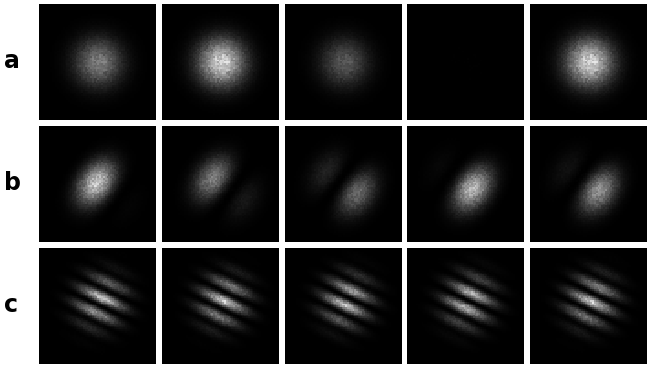
\includegraphics[width=0.8\linewidth]{images/visib_expl}
    }
    \caption{
    Interference images for various mirror positions obtained using a simulation program. (a) Perfectly aligned interferometer, visibility = 1; (b) Weakly misaligned interferometer, visibility = 0.3; (c) Highly misaligned interferometer, visibility = 0.0026. Images from left to right correspond to different points in time.}
\label{fig:visib_expl}
\end{figure}

The geometric dimensions of the interferometer used in the simulation and in the experiments are given in the table \ref{tab:interf_stat_params}. The focal lengths of lenses lens1 and lens2 are 50 mm. In the tuned state of the interferometer, the distance between the lenses is equal to the sum of the focal lengths. Lens lens1 is located at a distance of 50 mm from the beam splitter BS1.


\begin{table} [htbp]
    \centering
    \begin{threeparttable}% выравнивание подписи по границам таблицы
        \caption{Parameters of the interferometer, mm}
        \begin{tabular}{|c|c|c|c|c|}
            \hline
            \hline
            parameter   & length & width & distance to camera & beam radius \\
            \hline
            value & 200 & 300 & 100 & 0.71 \\
            \hline
            \hline
        \end{tabular}
        \label{tab:interf_stat_params}
    \end{threeparttable}
\end{table}

The maximum offsets from the aligned position for optical elements are given in the \ref{tab:interf_dyn_params} table. The values were chosen so as to reproduce the entire spectrum of interference patterns observed in the experiment.

\begin{table} [htbp]
    \centering
    \begin{threeparttable}% выравнивание подписи по границам таблицы
        \caption{The maximum offset value of each optical element. Mirror angles are in radians, lens positions are in millimeters.}
        \begin{tabular}{|c|c|c|c|c|c|}
            \hline
            \hline
            parameter & mirror 2, x & mirror 2, y & BS 2, x & BS 2, y & lens 2 \\
            \hline
            value & $2.6 \cdot 10^{-3}$ & $1.8 \cdot 10^{-3}$ & $1.3 \cdot 10^{-3}$ & $0.9 \cdot 10^{-3}$ & $7.5$ \\
            \hline
            \hline
        \end{tabular}
        \label{tab:interf_dyn_params}
    \end{threeparttable}
\end{table}


In the following sections we formulate the task of alignment of the interferometer in terms of reinforcement learning, present two agents trained with continuous and discrete action spaces, show evaluation results for the agents in the experimental setup. 

We view the interferometer alignment as a Markov decision process. The state of the environment $s$ is a sequence of 16 interference images obtained in one pass of the piezo mirror. The agent's actions must control the position of the optical elements of the interferometer. We implement this in the two ways --- specifying the action space as discrete and continuous. In the case of the discrete action space, the agent samples actions from a predetermined set of steps with different sizes. This allows the agent to use both large and small amplitude steps with equal confidence. In our implementation, the agent can change the positions of the optical elements independently and only in one direction at a time.  The agent was trained using the DQN \cite{dqn} algorithm. 
This method is simple but it limits the number of optical elements that the agent can operate simultaneously as well as speed of the interferometer alignment. To level this restrictions we  train second agent to align the interferometer using a continuous action space. In this case, the agent can operate simultaneously with all optical elements and change their position by an arbitrary value. The action of the agent $a$ is an N-dimensional vector $a \in (-1, 1)^{N}$. We use TD3 \cite{ddpg} algorithm to train the agent. Since at the end of the interferometer alignment the agent's actions become two orders of magnitude less than at the beginning, we need to rescale them:

\begin{equation}
a =
   \begin{cases}
    {\textrm sign}(a) \cdot 1000^{|a| - 1}  & \quad \text{if $|a| > 0.17$} 
    \\
    0  & \quad \text{if $|a| \leq 0.17$}
  \end{cases}
\end{equation}
Such a renormalization leads to actions in the interval $|a|\in\{0\}\cup[2.5 \cdot 10^{-3}, 1]$.

Next, we substantiate the choice of the reward function. The visibility of the interference pattern $V$ is not a good reward, as it does not allow the agent to differentiate states with $V$ close to 1, which is important in experiments. We chose the reward function $r = V - \log(1 - V)$. This reward function allows the agent to distinguish between the states which are closed to the aligned position. 

In order to transfer the trained agent on the experimental setup without substantial performance loss we trained it in simulation with environment randomizations based on the uncertainty of the setup parameters. At the beginning of each episode, we varied the beam radius by ±20\%, since this parameter is difficult to accurately measure. Changing the radius also helps to overcome the deviation of the experimental beam profile from the Gaussian distribution. The following randomizations were used at each step. First, we varied the brightness of the interference pattern by ±30\%, which simulates different camera exposure times. Second, we've added 20\% white noise to each pixel of the image, which can be seen as camera noise or dust on the camera \ref{fig:noise}. Thirdly, we added a cyclic shift of the interference images obtained in one pass of the piezo mirror and randomized the ratio of the times of forward and backward passes of the piezo mirror. The ratio of the number of images obtained during the forward pass was always greater than 50\%.

\begin{figure}[ht]
    \centerfloat{
        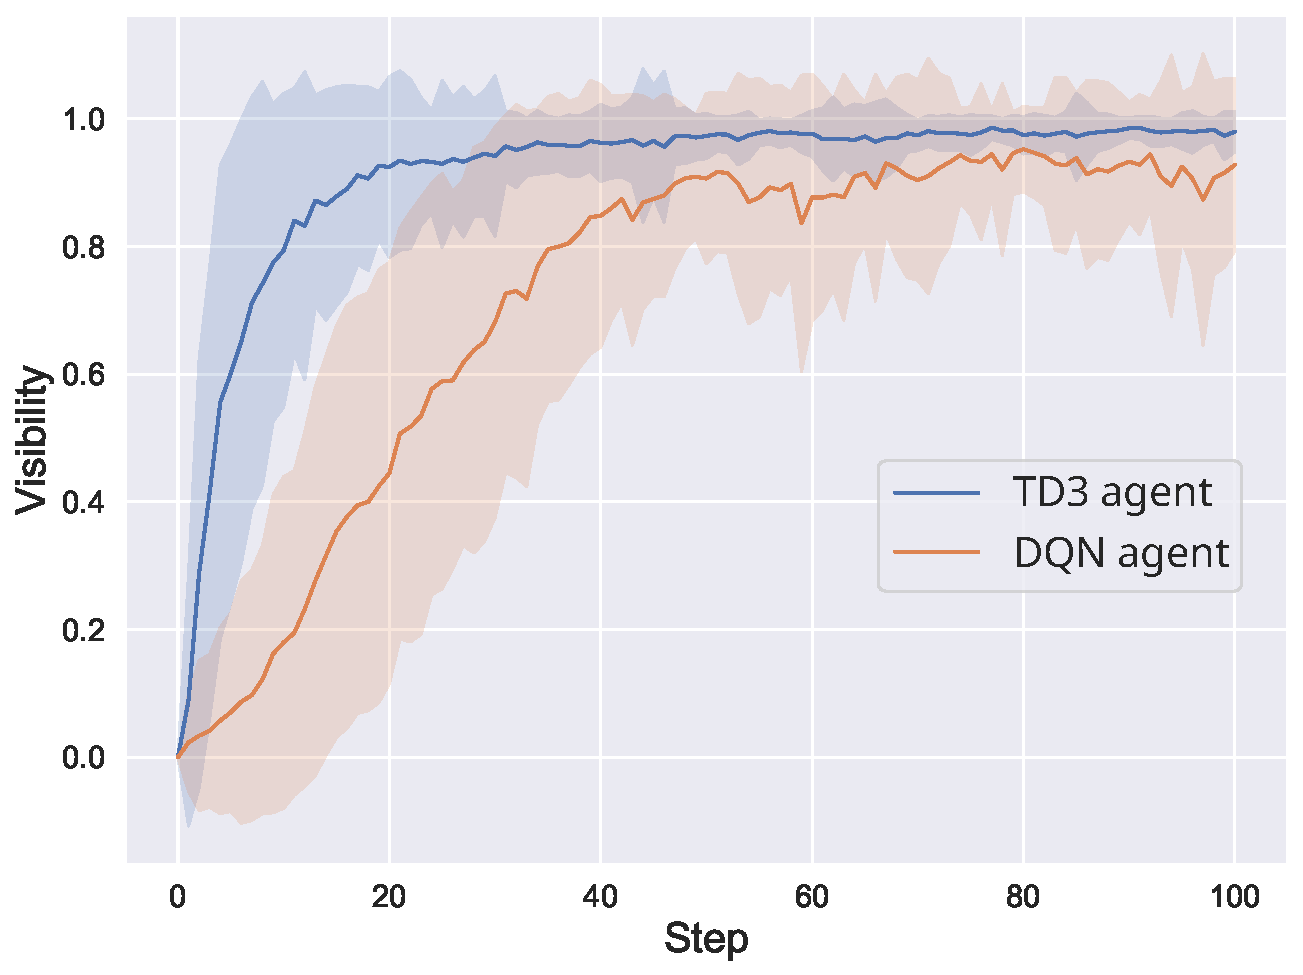
\includegraphics[width=0.8\linewidth]{images/dqn_vs_td3}
    }
    \caption{Evaluation of the agents on experimental setup.}\label{fig:interf_test}
\end{figure}

After, we describe the main characteristics of the developed hardware-software complex and present the results of evaluation of the agents on the experimental setup. We compare the quality of the interferometer alignment of the developed agents with an expert and an analyse the strategy used by agents when aligning the interferometer. The evaluation results are shown in the figure \ref{fig:interf_test}. The number of steps of the agent is plotted along the abscissa axis, the achieved visibility is plotted along the ordinate axis. Results are averaged over 100 episodes. From the figure \ref{fig:interf_test} it can be seen that both methods achieve a good value for the visibility of the interference pattern, but the TD3 agent which uses the continuous action space is faster and achieves better visibility than the DQN agent which operates in the discrete action space.

The evaluation results of the interferometer alignment by the developed methods are presented in the table \ref{tab:human}. It can be seen that the agent using the discrete action space works at the human level both in terms of the quality of the setting and in terms of speed. TD3 agent using a continuous action space aligns the interferometer much better than a human.

\begin{table} [htbp]
    \centering
    \begin{threeparttable}
        \caption{Comparison of the developed methods with an expert. The table shows the time required to achieve interference visibility of 0.92, 0.95 and 0.98. Percentage of episodes where this visibility was not achieved is shown in brackets.}
        \label{tab:human}
        \begin{tabular}{| p{2.5cm} || p{2.5cm} | p{2.5cm} | p{2.5cm} |}
            \hline
            \hline
            &V $\ge 0.92$ & V $\ge 0.95$ & V $\ge 0.98$\\
            \hline
            Expert &  93.9 (\textbf{0\%})  & 103.6 (\textbf{0\%}) & 129.6 (10\%)\\
            TD3 &  \textbf{56.16} (\textbf{0\%}) & \textbf{75.06} (\textbf{0\%}) & \textbf{120.1} (\textbf{4\%})\\
            DQN &  98.7 (7.6\%) & 116.1 (7.6\%) & 156.4 (10.6\%)\\
            \hline
            \hline
        \end{tabular}
    \end{threeparttable}
\end{table}

The results of the work were published in the articles \cite{confbib1, confbib2} at the leading scientific conferences <<Neural information processing systems (NeurIPS)>> and <<Conference on Robot Learning (CoRL)>> also the developed program was patented \cite{progbib1}.

\underline{\textbf{Chapter three}} is devoted to the development of a reinforcement learning method for motion control of the Unitree A1~\cite{unitree} robot. We developed a reward function that encourages the agent to learn safe and smooth movement strategy at a target speed. The agent was trained and tested in a simulation using the Raisim \cite{raisim} simulator. The agent was trained using the PPO~\cite{Schulman2017ProximalPO} algorithm as a backbone. We added a noise to the observations and applied a force to the torso of the robot in a random direction to force the agent to learn a stable moving policy during training. The observation space consists of the information about the orientation, speed of the robot, and the position and speed of its joints. The action space was continuous and each action corresponded to the desired position of the robot joints. Evaluation results are shown in tab.~\ref{tab:unitree_eval} and in fig.~ \ref{fig:unitree_eval_forward}. 

The table \ref{tab:unitree_eval} presents the evaluation results for the tasks ``Move forward'', ``Move backward'', ``Turn clockwise'' and ``Rotate counterclockwise''. It can be seen that for the tasks ``Move forward'', ``Move backward'' the learned policy is more stable and the number of steps is close to the maximum length of the episode. In the ``Turn Clockwise'' and ``Turn Counterclockwise'' tasks, the learned policy is less stable, resulting in lower overall rewards and lower average number of steps. The reason for this may be that the random force which was applied both during training and during testing  destabilizes a turning agent more than a one moving straight.

\begin{figure}[h]
\begin{subfigure}{.5\textwidth}
  \centering
  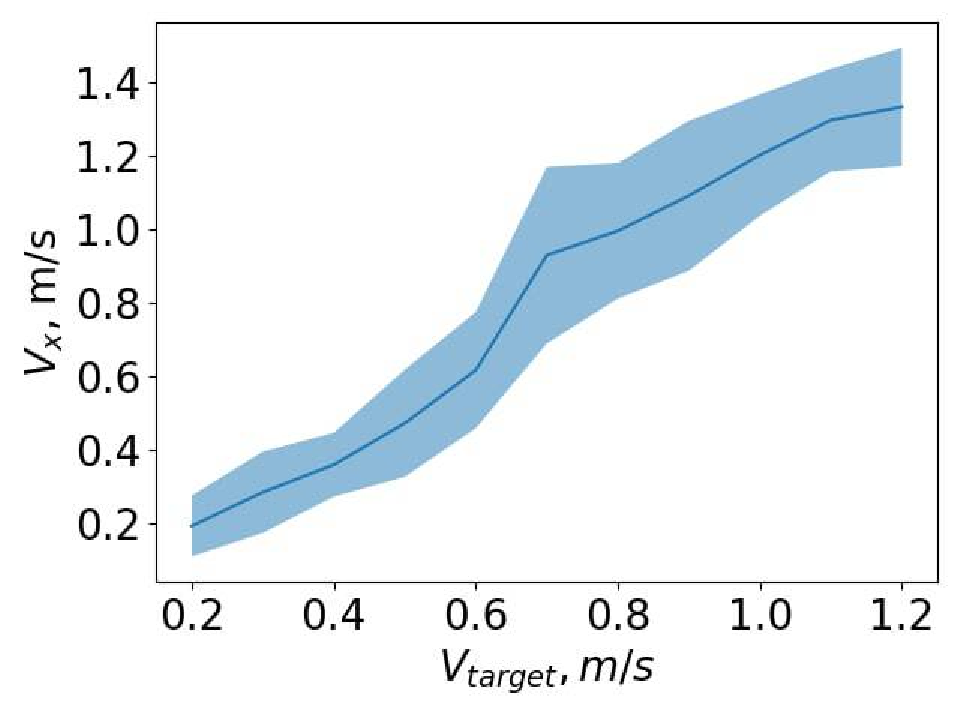
\includegraphics[width=1\textwidth]{images/vx}
\end{subfigure}%
\begin{subfigure}{.5\textwidth}
  \centering
  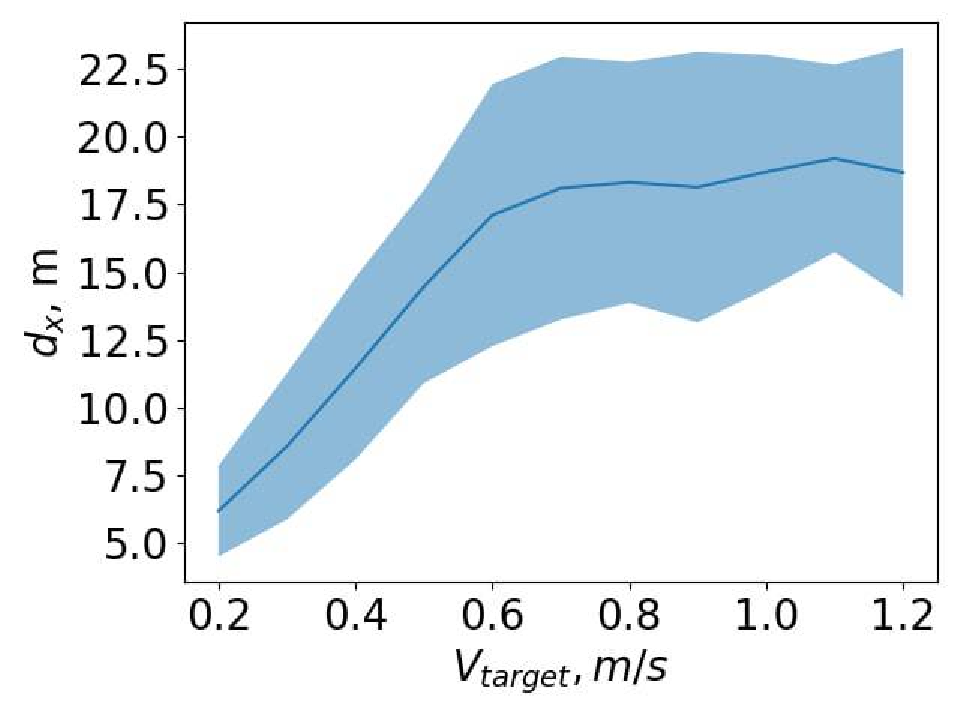
\includegraphics[width=1\textwidth]{images/dx}
\end{subfigure}%
\caption{Evaluation of the task ``Move forward at a given speed''. (a) Speed of the agent $V_x$ as a function of target speed $V_{target}$. (b) Distance traveled by the agent by the end of episode $d_x$ as a function of the target speed $V_{target}$.}
\label{fig:unitree_eval_forward}
\end{figure}

Figure~\ref{fig:unitree_eval_forward} shows the results of evaluation of the trained policy in the ``Move forward at a given speed'' task. It can be seen from fig.~\ref{fig:unitree_eval_forward}a that the trained agent is able to move at different speeds and the speed is close to the target speed. The distance traveled by the agent along the $x$ axis is shown in fig.~\ref{fig:unitree_eval_forward}b. At the target speed $V_{target} \in$ (0, 0.6) m/s, the distance traveled by the end of the episode increases. When the target speed is greater than 0.6 m/s, the distance traveled is almost constant and equal to the distance from the agent to the edge of the environment.

\begin{table} [htbp]
    \centering
    \begin{threeparttable}
        \caption{Evaluation results for the Unitree A1 robot in simulation}\label{tab:unitree_eval}
        \begin{tabular}{| p{2cm} || p{2cm} | p{2cm} | p{2cm} |p{2.5cm} |}
            \hline
            \hline
            Task & Move forward & Move backward & Turn clockwise & Turn counterclockwise \\
            \hline
            Return &	529 $\pm$ 124 &	508 $\pm$ 98 &	85 $\pm$ 219 &	165 $\pm$ 155 \\
            Number of steps & 3263 $\pm$ 633 &	3136 $\pm$ 545 &	2057 $\pm$ 1208 &	2095 $\pm$ 1325 \\
            \hline
            \hline
        \end{tabular}
    \end{threeparttable}
\end{table}

The obtained results show that the linear and angular speed of the Unitree A1 robot can be controlled by the proposed reinforcement learning method with a good quality.

\underline{\textbf{Четвертая глава}} посвящена исследованию методов машинного обучения с подкреплением для использования в среде Nethack. Среда Nethack основана на одноименной игре и предложена в качестве теста для алгоритмов машинного обучения в 2020 году \cite{nethack}. В этой игре агент путешествует по процедурно генерируемому подземелью. Игра имеет ascii интерфейс изображенный на рисунке \ref{fig:nethack}.

\begin{figure}[ht]
    \centerfloat{
        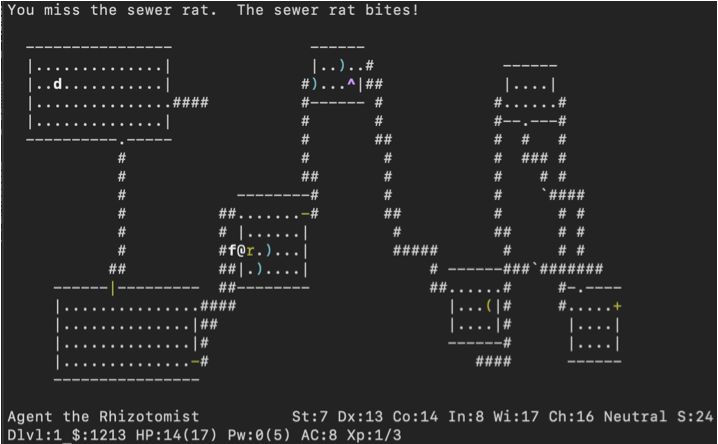
\includegraphics[width=0.8\linewidth]{images/nethack}
    }
    \caption{Игра Nethack}\label{fig:nethack}
\end{figure}

Основную сложность для алгоритмов обучения с подкреплением составляют сочетание различных типов данных в состоянии (изображения, текстовые описания, табличные данные), редкая функция награды и комбинаторно большое пространство действий. Для решения этой задачи нами был разработанный метод, сочетающий в себе машинное обучение с подкреплением, алгоритмы навигации на графах и алгоритмы, основанные на экспертных знаниях \ref{alg:raph}. Для решения различных подзадач возникающих в процесс игры таких как сражение с монстрами, исследование подземелья, обращение с предметами нами была реализована отдельная стратегия. Выбор стратегии на каждом шаге происходил в соответствии с их приоритетом заданным вручную. Стратегия сражения с монстрами обучалась с помощью алгоритма IMPALA \cite{impala} и имела дискретное пространство действий. Остальные стратегии были реализованы с использованием алгоритмов навигации на графах. Данный подход позволил превзойти остальные подходы с использованием обучения с подкреплением в этой задаче. Результаты были опубликованы на одной из ведущих конференции по машинному обучению NeurIPS в рамках трека посвященного соревнованиям \cite{confbib3}.


\begin{algorithm}[ht]
\SetKwComment{Comment}{/* }{ */}
\SetKw{Continue}{continue}
\caption{RAPH agent}\label{alg:raph}
\KwData{view\_distance, agent, hard\_coded\_skills}
$state, done \gets env.reset(), False$\;

\While{not done}{
  action\_queue = parse\_message(state)\;

  \If{action\_queue} {
   state, reward, done, info = env.step(action\_queue)\Comment*[r]{We have a prompt to response}
   \Continue
  }

  monster\_distance, preprocessed\_state = parse\_dungeon(state)\;
  \eIf{monster\_distance \textless view\_distance}{
    action\_queue = agent.act(preprocessed\_state)\;
  }{
    action\_queue = first\_fit(hard\_coded\_skills, preprocessed\_state)\Comment*[r]{Select non-rl action on first-fit basis}
  }
  state, reward, done, info = env.step(action\_queue)\;
}
\end{algorithm}


\FloatBarrier
\section*{\centering CONCLUSION}
\pdfbookmark{Заключение}{conclusion}                                  % Закладка pdf
В \underline{\textbf{заключении}} приведены основные результаты работы, которые заключаются в следующем:
%% Согласно ГОСТ Р 7.0.11-2011:
%% 5.3.3 В заключении диссертации излагают итоги выполненного исследования, рекомендации, перспективы дальнейшей разработки темы.
%% 9.2.3 В заключении автореферата диссертации излагают итоги данного исследования, рекомендации и перспективы дальнейшей разработки темы.
\begin{enumerate}
  \item Была разработанна компьютерная модель оптического интерферометра Маха-Цендера. Процесс настройки интерферометра был представлен в виде марковского процесса принятия решений на основании которого была разработана среда для обучения агентов машинного обучения с подкреплением по настройке оптического интерферометра. 
  \item На основе среды были разработаны методы основанные на обучении с подкреплением, которые позволили выучить алгоритм настройки интерферометра по изображениям с камеры. 
  \item Разработанные методы были успешно протестированы при настройке экспериментальной установки интерферометра. 
  \item Был разработан метод включающий в себя обучения с подкреплением для управлением виртуальным агентом в среде Nethack. 
\end{enumerate}

\newpage


\pdfbookmark{Литература}{bibliography}                                % Закладка pdf

\ifdefmacro{\microtypesetup}{\microtypesetup{protrusion=false}}{} % не рекомендуется применять пакет микротипографики к автоматически генерируемому списку литературы
\urlstyle{rm}                               % ссылки URL обычным шрифтом
\ifnumequal{\value{bibliosel}}{0}{% Встроенная реализация с загрузкой файла через движок bibtex8
}{% Реализация пакетом biblatex через движок biber
    % Цитирования.
    %  * Порядок перечисления определяет порядок в библиографии (только внутри подраздела, если `\insertbiblioauthorgrouped`).
    %  * Если не соблюдать порядок "как для \printbibliography", нумерация в `\insertbiblioauthor` будет кривой.
    %  * Если цитировать каждый источник отдельной командой --- найти некоторые ошибки будет проще.
    %

    \insertbiblioexternal            % Вывод списка литературы, на которую ссылались в тексте автореферата
}
\ifdefmacro{\microtypesetup}{\microtypesetup{protrusion=true}}{}
\urlstyle{tt}                               % возвращаем установки шрифта ссылок URL
